\documentclass[border=12pt]{standalone}
\usepackage{tikz,amsmath}
\usepackage[scaled]{helvet}
\renewcommand{\familydefault}{\sfdefault}
\usetikzlibrary{arrows.meta,positioning,calc,decorations.pathreplacing,patterns}
\definecolor{pro}{HTML}{1F5FA8}\definecolor{limb}{HTML}{C2410C}\definecolor{hot}{HTML}{DC2626}
\definecolor{good}{HTML}{15803D}\definecolor{ink}{HTML}{1F2937}\definecolor{quiet}{HTML}{6B7280}
\tikzset{>=Stealth,every node/.style={text=ink}}

\begin{document}
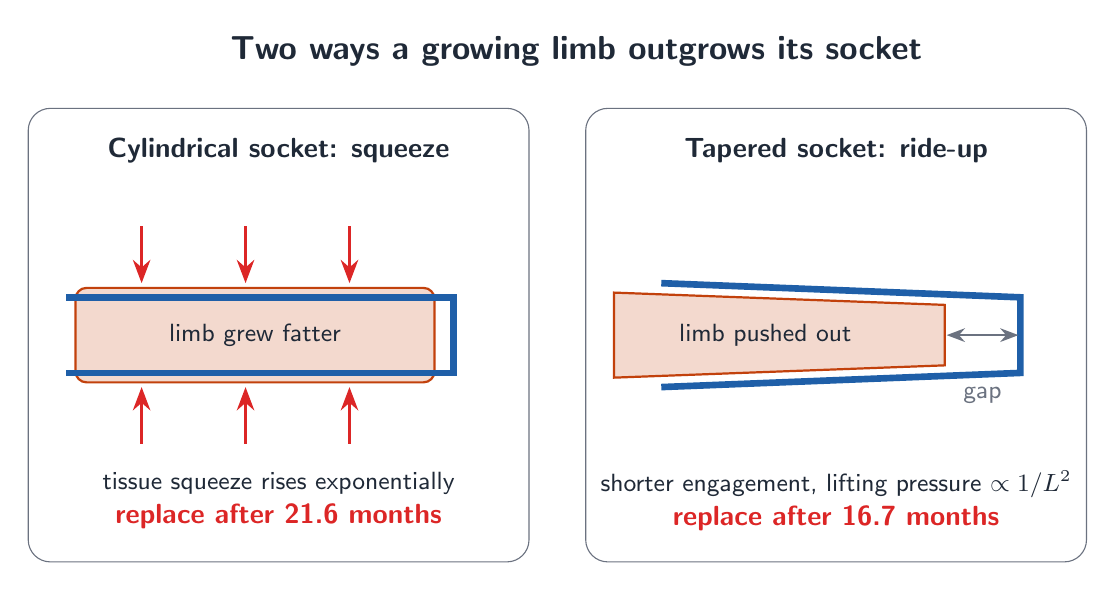
\begin{tikzpicture}[scale=1.2]
\node[font=\large\bfseries] at (5.4,3.0) {Two ways a growing limb outgrows its socket};
\draw[quiet,rounded corners=8pt] (-0.4,-2.4) rectangle (4.9,2.4);
\node[font=\bfseries] at (2.25,1.95) {Cylindrical socket: squeeze};
\fill[limb!20,draw=limb,thick,rounded corners=4pt] (0.1,-0.5) rectangle (3.9,0.5);
\draw[pro,line width=2.4pt] (0,0.4)--(4.1,0.4)--(4.1,-0.4)--(0,-0.4);
\foreach \x in {0.8,1.9,3.0} {\draw[->,hot,very thick] (\x,1.15)--(\x,0.55); \draw[->,hot,very thick] (\x,-1.15)--(\x,-0.55);}
\node at (2.0,0) {\small limb grew fatter};
\node[align=center] at (2.25,-1.75) {\small tissue squeeze rises exponentially\\\textcolor{hot}{\bfseries replace after 21.6 months}};
\begin{scope}[xshift=5.9cm]
\draw[quiet,rounded corners=8pt] (-0.4,-2.4) rectangle (4.9,2.4);
\node[font=\bfseries] at (2.25,1.95) {Tapered socket: ride-up};
\fill[limb!20,draw=limb,thick] (-0.1,0.45)--(3.4,0.32)--(3.4,-0.32)--(-0.1,-0.45)--cycle;
\draw[pro,line width=2.4pt] (0.4,0.55)--(4.2,0.4)--(4.2,-0.4)--(0.4,-0.55);
\draw[<->,thick,quiet] (3.42,0)--(4.18,0); \node[quiet,below] at (3.8,-0.45) {\small gap};
\node at (1.5,0) {\small limb pushed out};
\node[align=center] at (2.25,-1.75) {\small shorter engagement, lifting pressure $\propto 1/L^2$\\\textcolor{hot}{\bfseries replace after 16.7 months}};
\end{scope}
\end{tikzpicture}
\end{document}
